

\subsubsection{Aktivität u00 - Hauptmenü}

\vspace*{1cm}

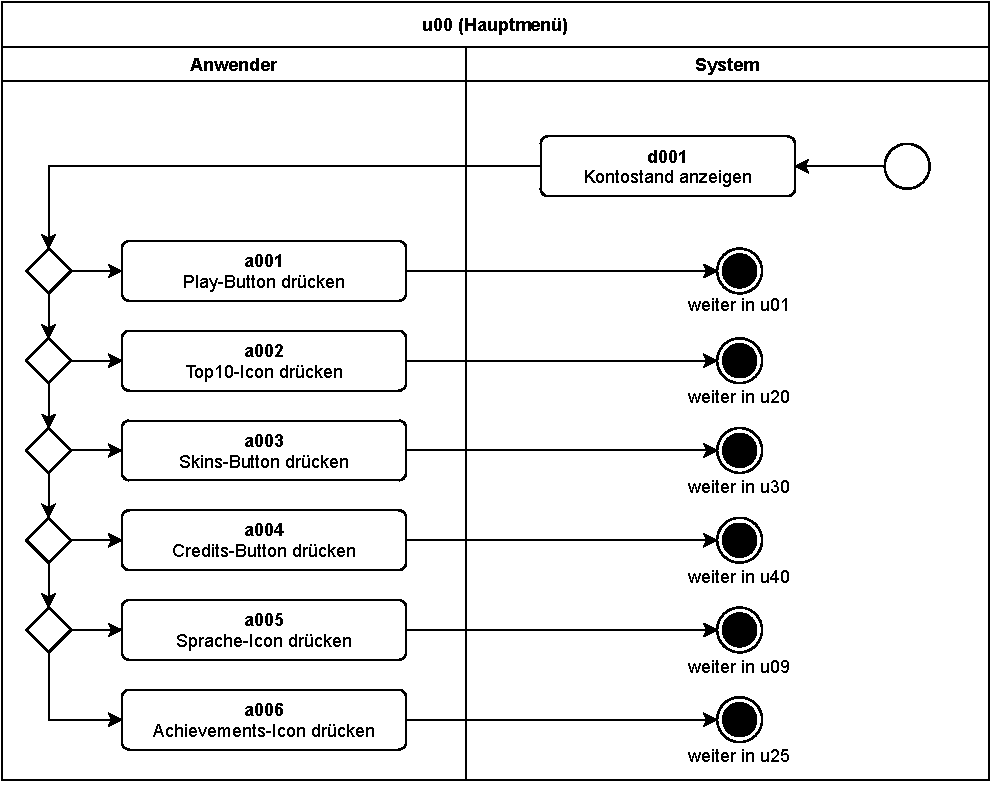
\includegraphics[width=\linewidth]{diagramme/pdf/UML-Activity-u00.pdf}
\captionof{figure}{Aktivität u00 - Hauptmenü}\label{fig:dia:mainMenu}
\vspace*{0.5cm}


Im \hyperref[fig:dia:mainMenu]{Hauptmenü} stehen dem \gls{spieler} fünf verschiedene Buttons zur Verfügung, die ihn zu anderen Screens leiten. Mit dem Play-Button gelangt man zur Spielauswahl. Über den \gls{Top10} Button kann man sich die Zehn besten Spieldurchläufe im \gls{classicMode} und \gls{invasionMode} anschauen. Im Spiel sind außerdem \gls{skin}s enthalten, die man nach Klicken des Skins-Buttons anschauen und kaufen kann. Mit dem Credits-Button gelangt man zu einem Screen, der ein paar Worte der Entwickler enthält und alle Mitwirkenden am Spiel auflistet. Über das Sprache-Icon öffnet sich ein Overlay direkt über dem \hyperref[fig:dia:mainMenu]{Hauptmenü}, dass dem \gls{spieler} die Möglichkeit gibt, die Sprache der gesamten App zu ändern. Die Standard-Sprache ist Englisch. Zuletzt gibt es noch ein weiteres Fenster für Achievements, das über das Achievements-Icon aufgerufen werden kann.


\clearpage

\subsubsection{Aktivität u01 - Spielmodus Einstellungen}

\vspace*{1cm}
   
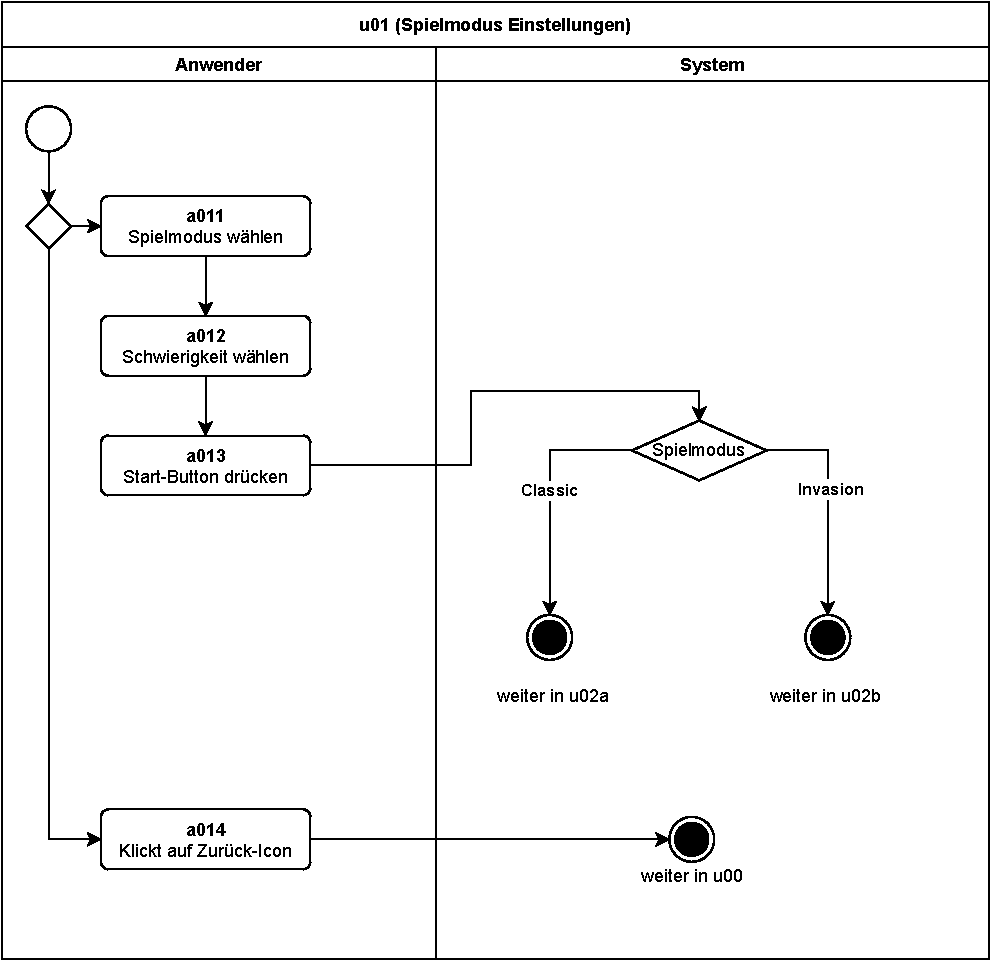
\includegraphics[width=\linewidth]{diagramme/pdf/UML-Activity-u01.pdf}
\captionof{figure}{Aktivität u01 - Spielmodus Einstellungen}\label{fig:dia:gameMode}
\vspace*{0.5cm}


Hat der \gls{spieler} den Play-Button gedrückt, so gelangt er in ein neues Fenster, dass ihm die Möglichkeit bietet, den Spielmodus (\gls{classicMode}/\gls{invasionMode}) und die Schwierigkeit (Easy, Medium, Hard) einzustellen. Drückt der \gls{spieler} dann den Start Button, wird eine neue Spielrunde mit den ausgewählten Einstellungen geladen. Über das Zurück-Icon gelangt man wieder in das \hyperref[fig:dia:mainMenu]{Hauptmenü} und die Einstellungen werden verworfen.

\clearpage

\subsubsection{Aktivität u02a - Spiel Classic}

\vspace*{1cm}

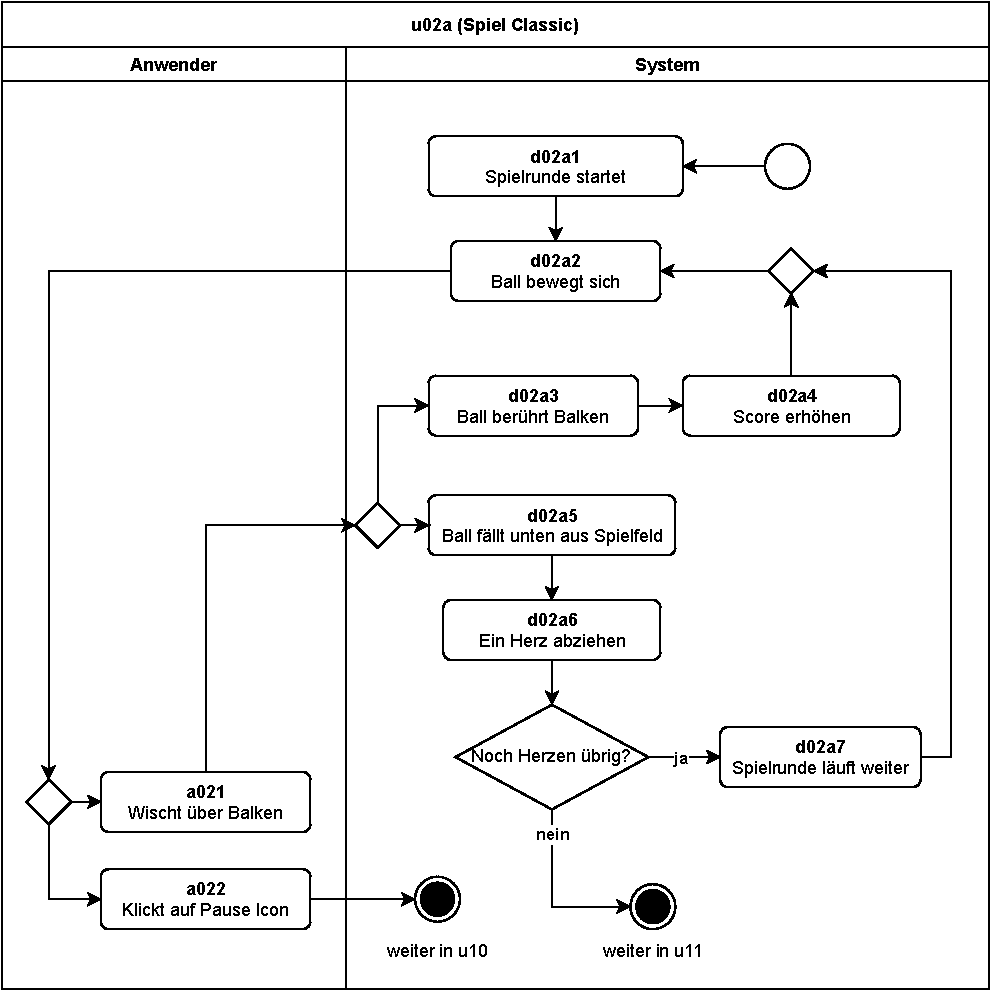
\includegraphics[width=\linewidth]{diagramme/pdf/UML-Activity-u02a.pdf}
\captionof{figure}{Aktivität u02a - Spiel Classic}\label{fig:dia:classic}
\vspace*{0.5cm}


Im \gls{classicMode} muss der \gls{spieler} den \gls{ball} mithilfe des \gls{balken} im \gls{spielfeld} halten, indem er diesen durch Wischen auf dem Screen nach links und rechts bewegt. Berührt der \gls{ball} den \gls{balken}, die Wände oder Decke des Spielfelds, so prallt er ab und ändert seine Richtung abhängig vom Auftreffwinkel. Außerdem wird der Score jedes Mal erhöht, wenn der \gls{ball} den \gls{balken} trifft.
Fällt der Ball unten aus dem \gls{spielfeld}, so verliert der Spieler ein Herz (Startet mit 3), der \gls{ball} wird wieder in die Mitte gesetzt und die Runde läuft weiter. Sollte der \gls{spieler} jedoch drei Herzen verlieren, so ist die Runde vorläufig zu Ende und der Game-Over Screen wird aufgerufen.
Der Spieler hat jedoch während der gesamten Zeit immer die Möglichkeit zu pausieren und gegebenenfalls die Runde frühzeitig zu beenden.  


\clearpage
\subsubsection{Aktivität u02b - Spiel Invasion}

\vspace*{1cm}

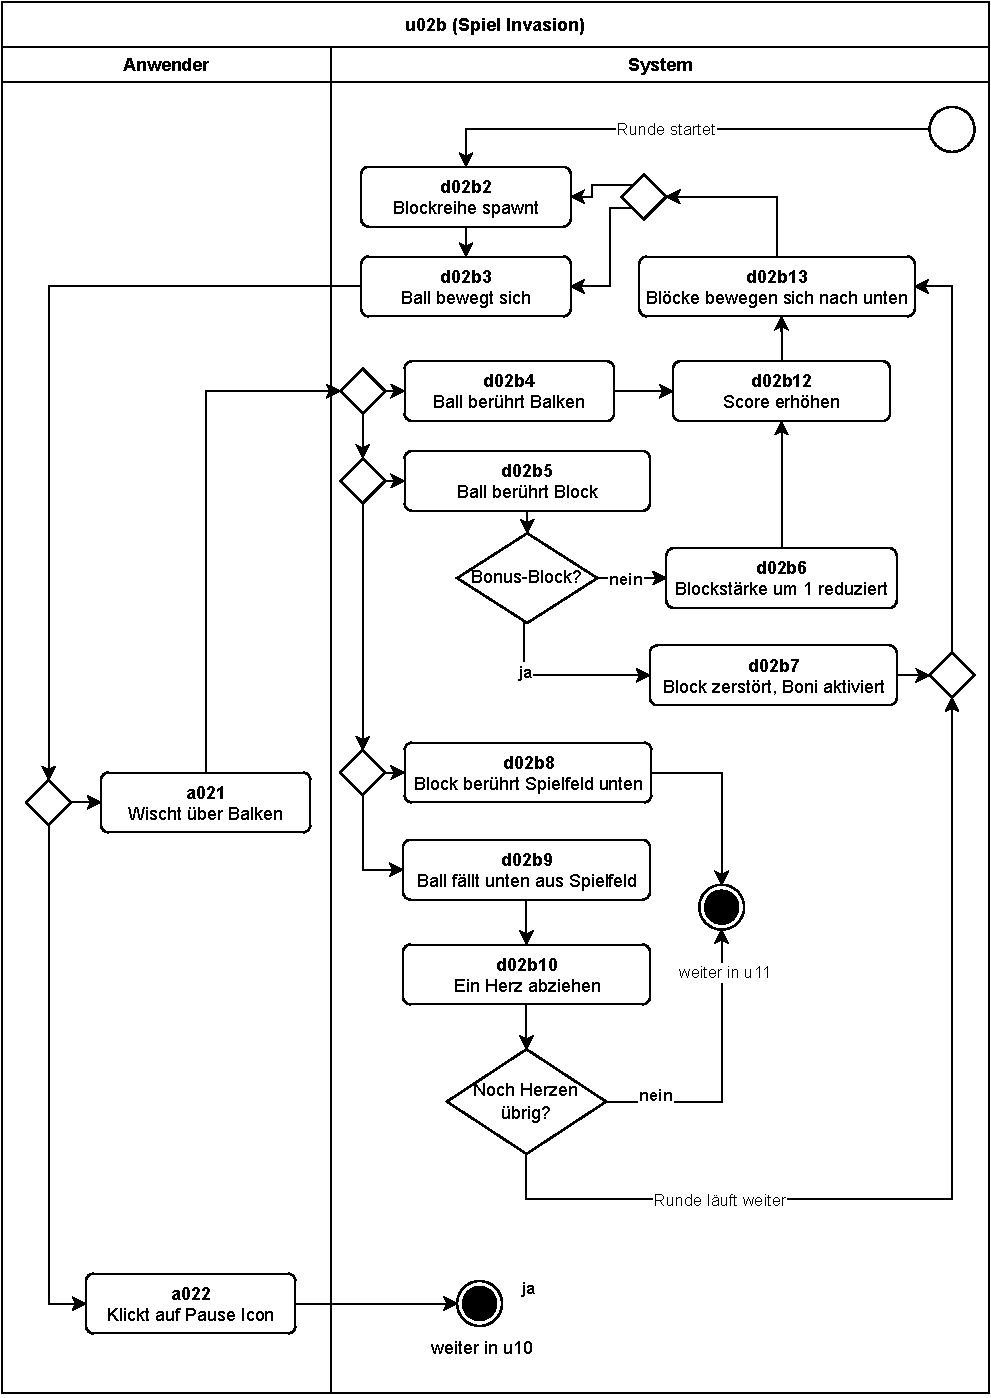
\includegraphics[width=\linewidth]{diagramme/pdf/UML-Activity-u02b.pdf}
\captionof{figure}{Aktivität u02b - Spiel Invasion}\label{fig:dia:invasion}
\vspace*{0.5cm}


Der \gls{invasionMode} ist eine Erweiterung zum \gls{classicMode}. Ab Rundenstart spawnt periodisch eine Reihe an Blöcken verschiedener Stärke und vereinzelt mit Boni für den \gls{spieler}. Diese Blöcke müssen mehrmals (abhängig von der Stärke des Blocks) vom \gls{ball} getroffen werden, um sie zu zerstören. Zerstört der Spieler einen Bonus-\gls{block}, so erhält der \gls{ball} (oder der \gls{spieler}) für kurze Zeit eine besondere Eigenschaft. (Siehe 9.2.1). 
Alle anderen Spielabläufe des \gls{invasionMode} sind identisch zu dem des \gls{classicMode} (5.1.3).


\clearpage

\subsubsection{Aktivität u09 - Sprachauswahl}

\vspace*{1cm}

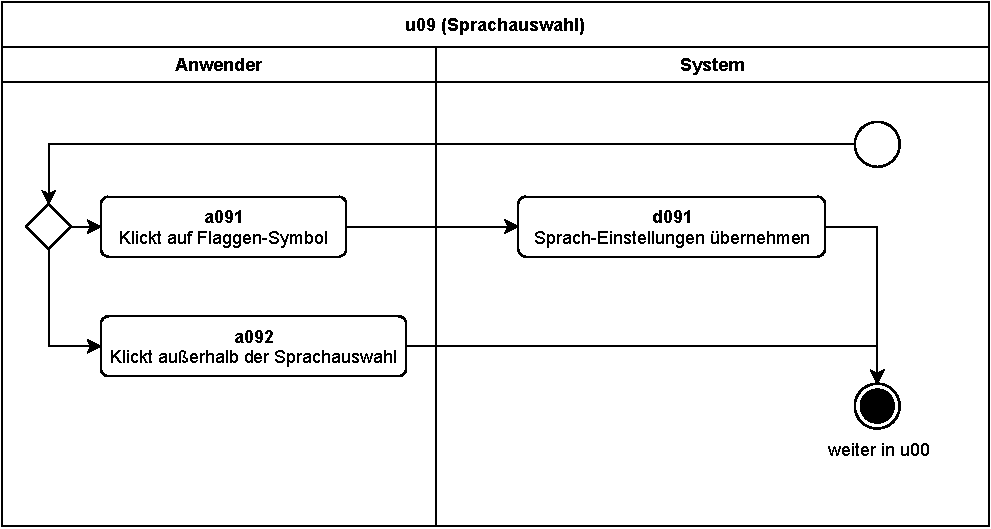
\includegraphics[width=\linewidth]{diagramme/pdf/UML-Activity-u09.pdf}
\captionof{figure}{Aktivität u09 - Sprachauswahl}\label{fig:dia:language}
\vspace*{0.5cm}



Wurde das Sprache-Icon im Hauptmenü gedrückt, öffnet sich ein Overlay. Darin hat der \gls{spieler} die Möglichkeit die Sprache des Spiels zu ändern, indem er auf eine der verfügbaren Flaggen klickt. Die Standardeinstellung der Sprache ist Englisch. Durch das Klicken außerhalb der Sprachauswahl kommt der \gls{spieler} wieder in das \hyperref[fig:dia:mainMenu]{Hauptmenü} zurück.

\clearpage

\subsubsection{Aktivität u09 - Achievements}

\vspace*{1cm}

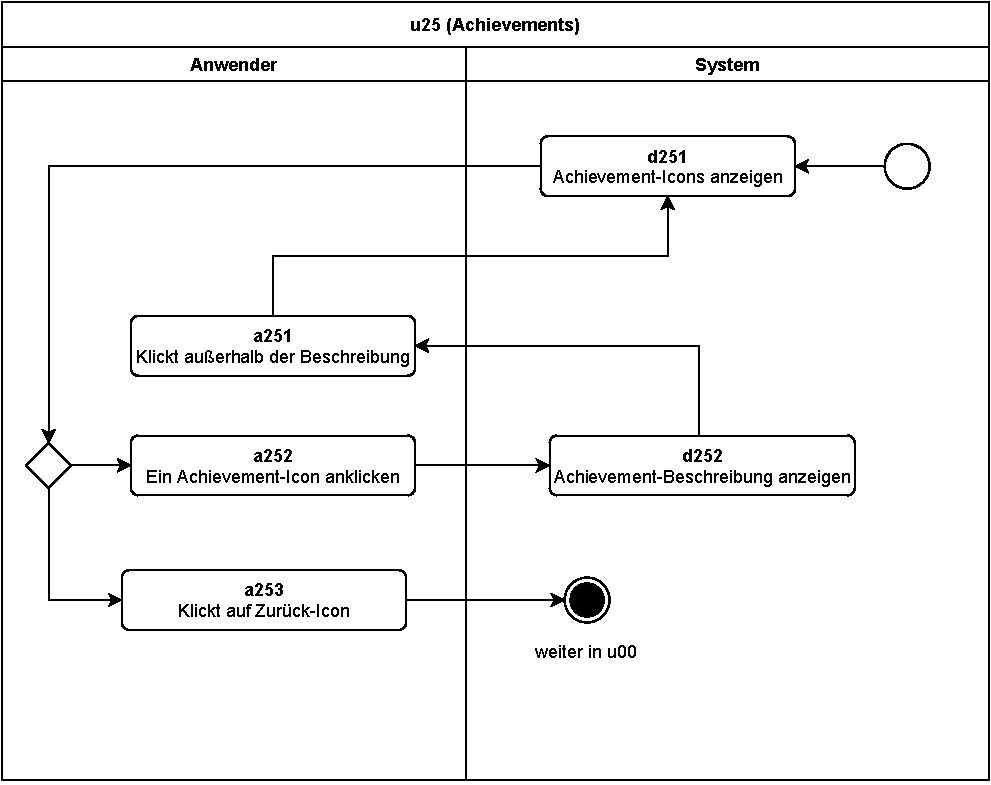
\includegraphics[width=\linewidth]{diagramme/pdf/UML-Activity-u25.pdf}
\captionof{figure}{Aktivität u25 - Achievements}\label{fig:dia:achievements}
\vspace*{0.5cm}

Über das Achievements-Icon gelangt der \gls{spieler} auf einen Screen, der alle seine bisher erreichten Achievements anzeigt (Noch nicht erreichte sind ausgegraut sein). Wird auf eines der Icons geklickt, so öffnet sich ein Overlay und der Spieler kann die Beschreibung des jeweiligen Achievements nachlesen. Durch das Klicken des Zurück-Icons gelangt der Spieler dann wieder in das \hyperref[fig:dia:mainMenu]{Hauptmenü}. 

\clearpage

\subsubsection{Aktivität u10 - Pause Menü}


\vspace*{1cm}

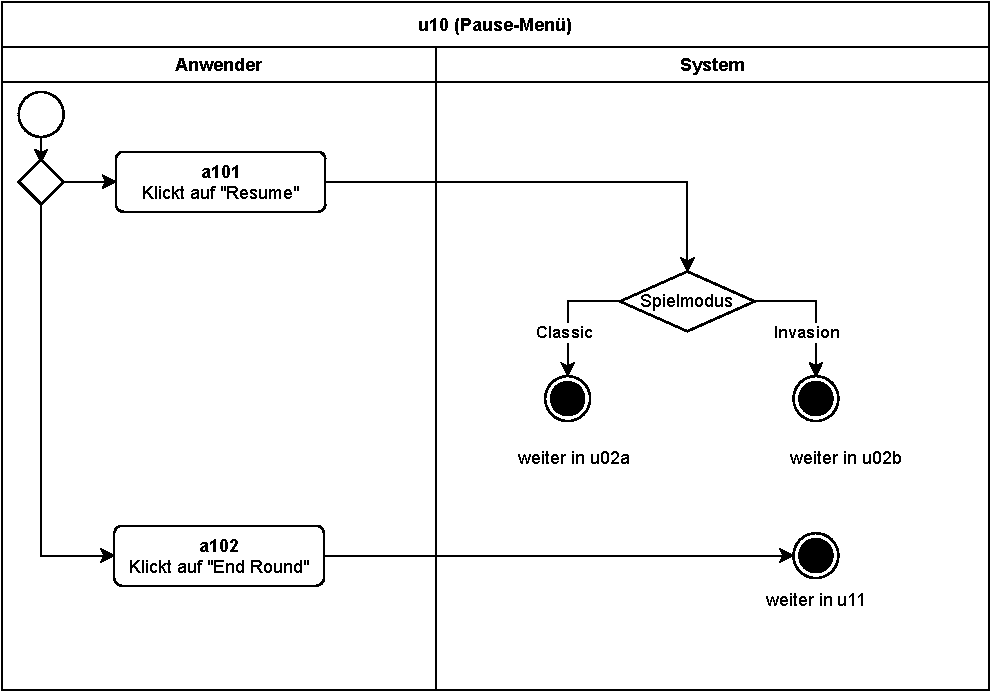
\includegraphics[width=\linewidth]{diagramme/pdf/UML-Activity-u10.pdf}
\captionof{figure}{Aktivität u10 - Pause Menü}\label{fig:dia:pause}
\vspace*{0.5cm}


Während einer aktiven Spielrunde hat der \gls{spieler} die Möglichkeit zu pausieren. Dann wird das Spiel angehalten und ein Overlay öffnet sich. Darin kann der Spieler entweder den Resume Button klicken, um die jeweilige Runde fortzusetzen, oder auf End Round klicken, um die Runde frühzeitig zu beenden.

\clearpage

\subsubsection{Aktivität u11 - Game-Over-Menü}

\vspace*{1cm}

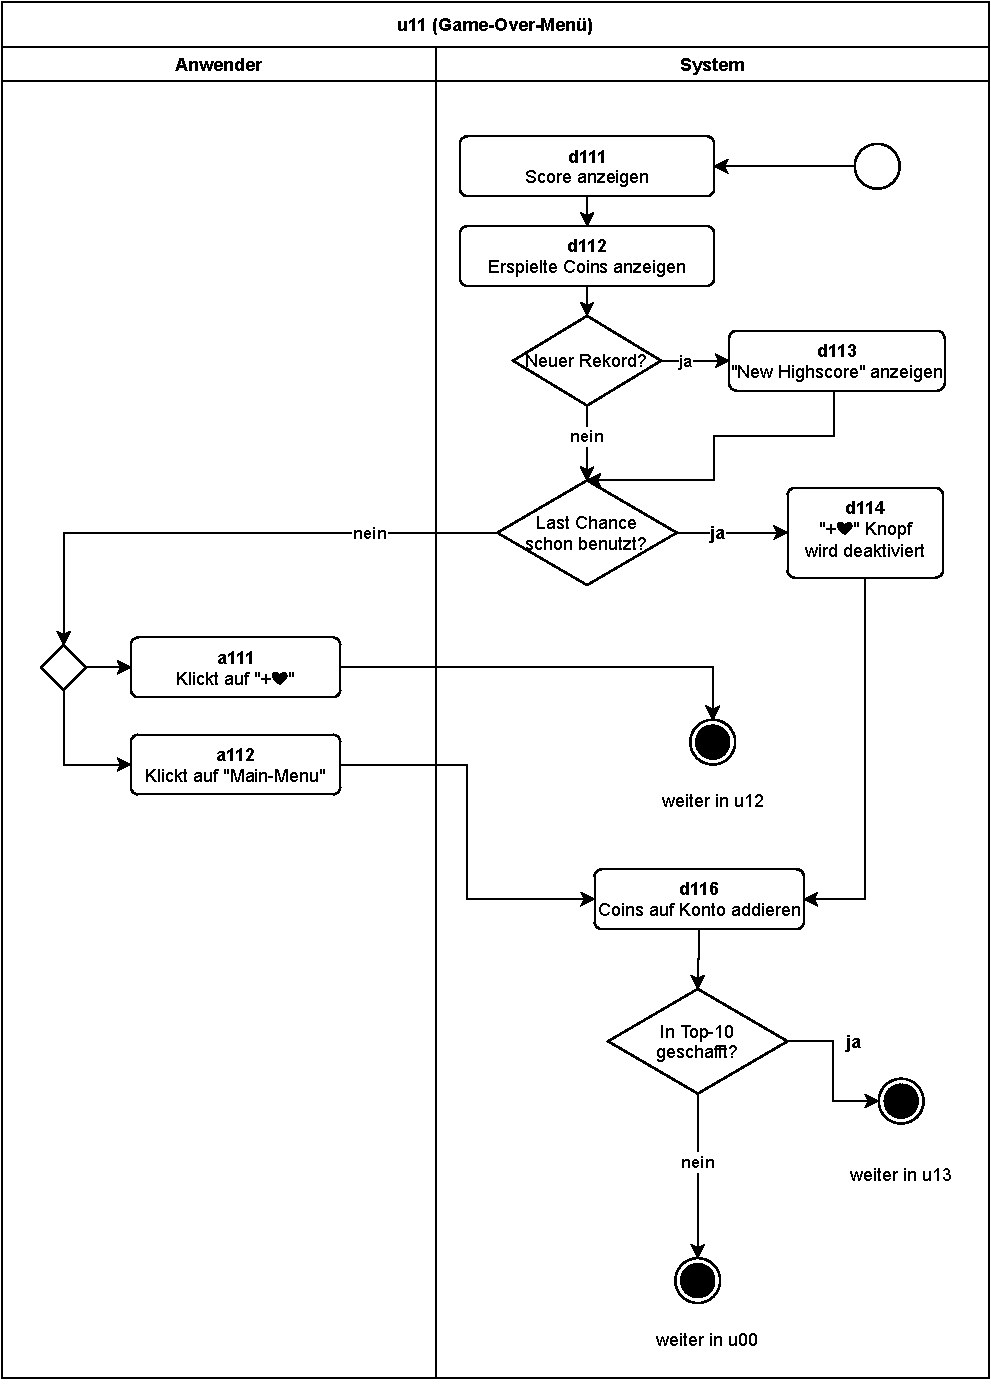
\includegraphics[width=\linewidth]{diagramme/pdf/UML-Activity-u11.pdf}
\captionof{figure}{Aktivität u11 - Game-Over-Menü}\label{fig:dia:gameOver}
\vspace*{0.5cm}


Hat der \gls{spieler} alle seine Herzen verloren, oder die Runde im Pause Menü frühzeitig beendet, so kommt er automatisch in das Game-Over Menü. Hier sieht er den bisher erreichten Score und die erspielten Coins. Hat er in der Runde einen höheren Score erreicht als der erste Platz in der \gls{Top10} Liste, bekommt der \gls{spieler} die Nachricht „new Highscore“ auf dem Screen angezeigt. Hat der \gls{spieler} noch keine „last Chance“ genutzt, so bietet ihm das System einmalig die Möglichkeit, einen Werbeclip zu schauen, um nochmal ein Herz zu erhalten und die Runde fortzusetzen. Verliert der \gls{spieler} auch dieses Herz ist die Runde endgültig zu Ende. Danach werden die erspielten Coins automatisch auf das Spiel-Konto addiert und das System prüft, ob der Score des Spielers hoch genug ist um in die \gls{Top10} zu kommen. Ist dies der Fall, so wird eine Namenseingabe angezeigt, in der der \gls{spieler} seinen Namen eingeben kann. Hat der \gls{spieler} keine \gls{Top10} Platzierung erreicht, wird das \hyperref[fig:dia:mainMenu]{Hauptmenü} geöffnet.
\clearpage

\subsubsection{Aktivität u12 - Werbung}

\vspace*{1cm}

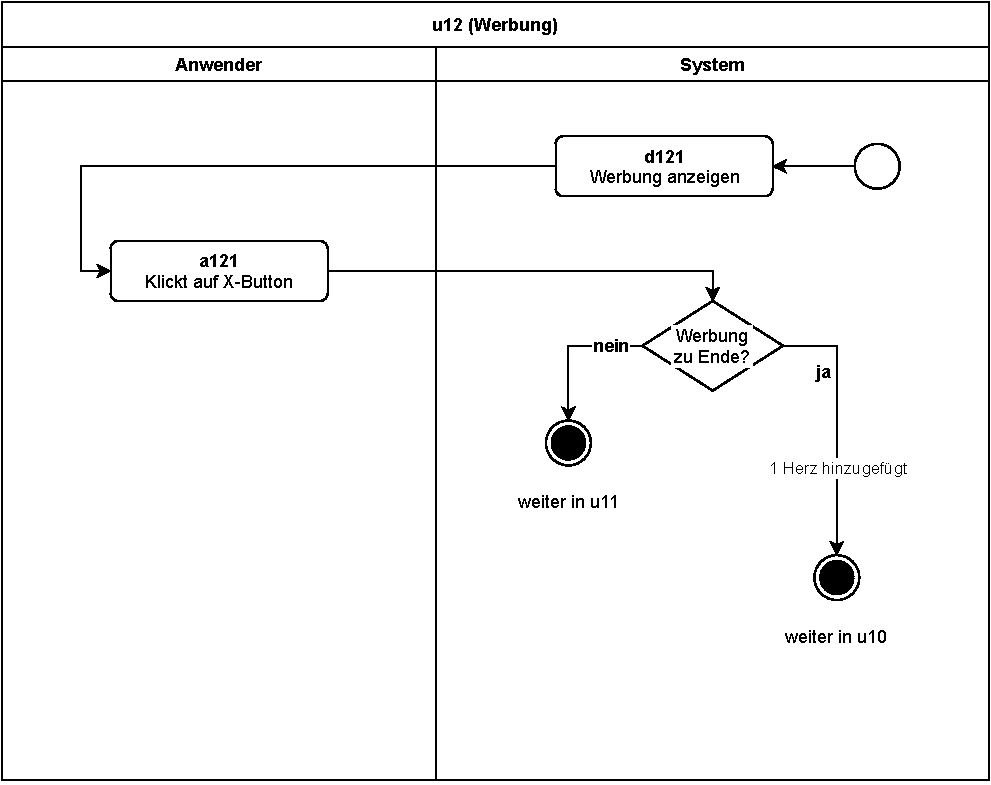
\includegraphics[width=\linewidth]{diagramme/pdf/UML-Activity-u12.pdf}
\captionof{figure}{Aktivität u12 - Werbung}\label{fig:dia:ads}
\vspace*{0.5cm}

Entscheidet sich der \gls{spieler} Werbung anzuschauen, so hat er die Möglichkeit, diese über den „X“ Button wieder zu schließen. Ist die Werbung zu diesem Zeitpunkt noch nicht vollständig durchgelaufen, so wird der \gls{spieler} wieder in das Game-Over Menü weitergeleitet. Hat er sich die Werbung jedoch vollständig angeschaut, so erhält er ein extra Herz und wird zum Pause Menü weitergeleitet, sodass die Runde fortgesetzt werden kann.

\clearpage

\subsubsection{Aktivität u13 - Namenseingabe}

\vspace*{1cm}

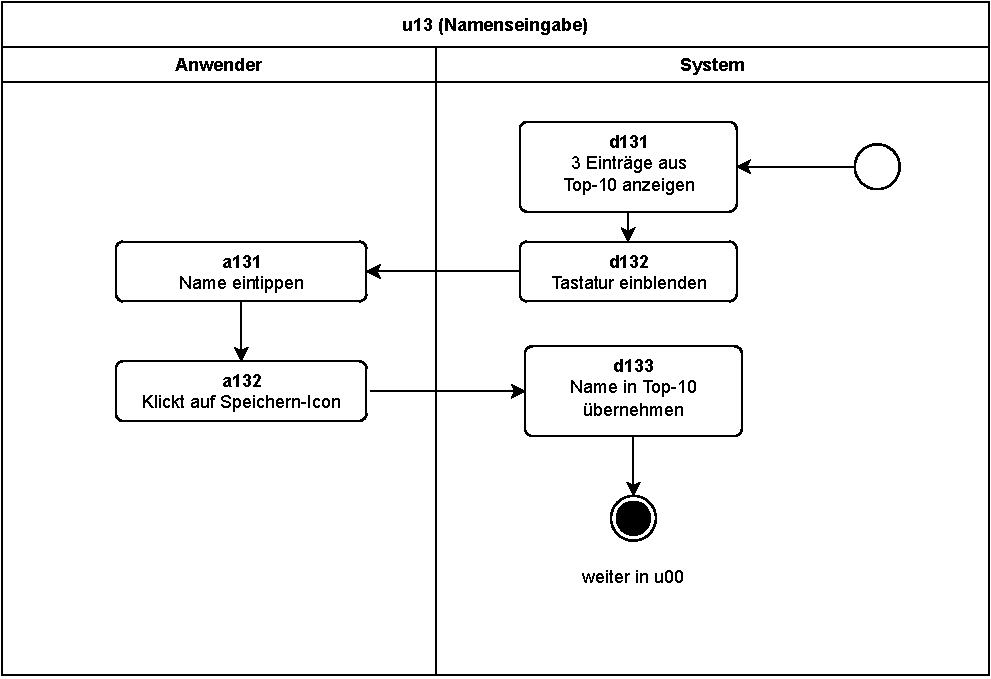
\includegraphics[width=\linewidth]{diagramme/pdf/UML-Activity-u13.pdf}
\captionof{figure}{Aktivität u13 - Namenseingabe}\label{fig:dia:highscore}
\vspace*{0.5cm}

Hat der \gls{spieler} nach der Runde eine \gls{Top10} Platzierung erreicht, so wird die Namenseingabe angeboten. Es werden, sofern vorhanden, drei Einträge der Platzierungen genau vor dem des erreichten Scores angezeigt. Unterhalb dieser Anzeige wird die Tastatur
eingeblendet und der \gls{spieler} hat so die Möglichkeit seinen Namen einzutippen und anschließend durch den Klick auf das Speichern-Icon seinen Namen in den \gls{Top10} zu sichern. Danach wird der \gls{spieler} wieder in das \hyperref[fig:dia:mainMenu]{Hauptmenü} geleitet.

\clearpage

\subsubsection{Aktivität u20 - Top-10 Liste}

\vspace*{1cm}

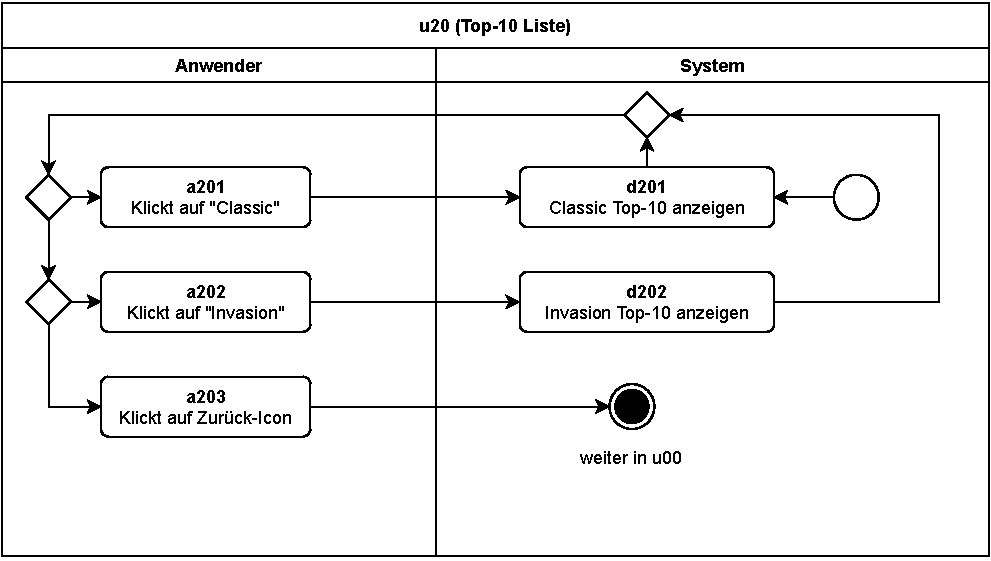
\includegraphics[width=\linewidth]{diagramme/pdf/UML-Activity-u20.pdf}
\captionof{figure}{Aktivität u20 - Top-10 Liste}\label{fig:dia:top10}
\vspace*{0.5cm}

Klickt der \gls{spieler} im \hyperref[fig:dia:mainMenu]{Hauptmenü} auf den \gls{Top10} Button, so werden ihm standardmäßig die 10 höchsten Scores im \gls{classicMode} in Listenform angezeigt. Durch einen klick auf den Invasion-Button ändert sich die Liste und zeigt dann die 10 höchsten Scores im \gls{invasionMode}. Analog dazu führt der Classic-Button zur Top-10 Liste des \gls{classicMode} zurück.
Über das Zurück-Icon gelangt der \gls{spieler} wieder in das \hyperref[fig:dia:mainMenu]{Hauptmenü}.

\clearpage

\subsubsection{Aktivität u30 - Skin-Auswahl}

\vspace*{1cm}

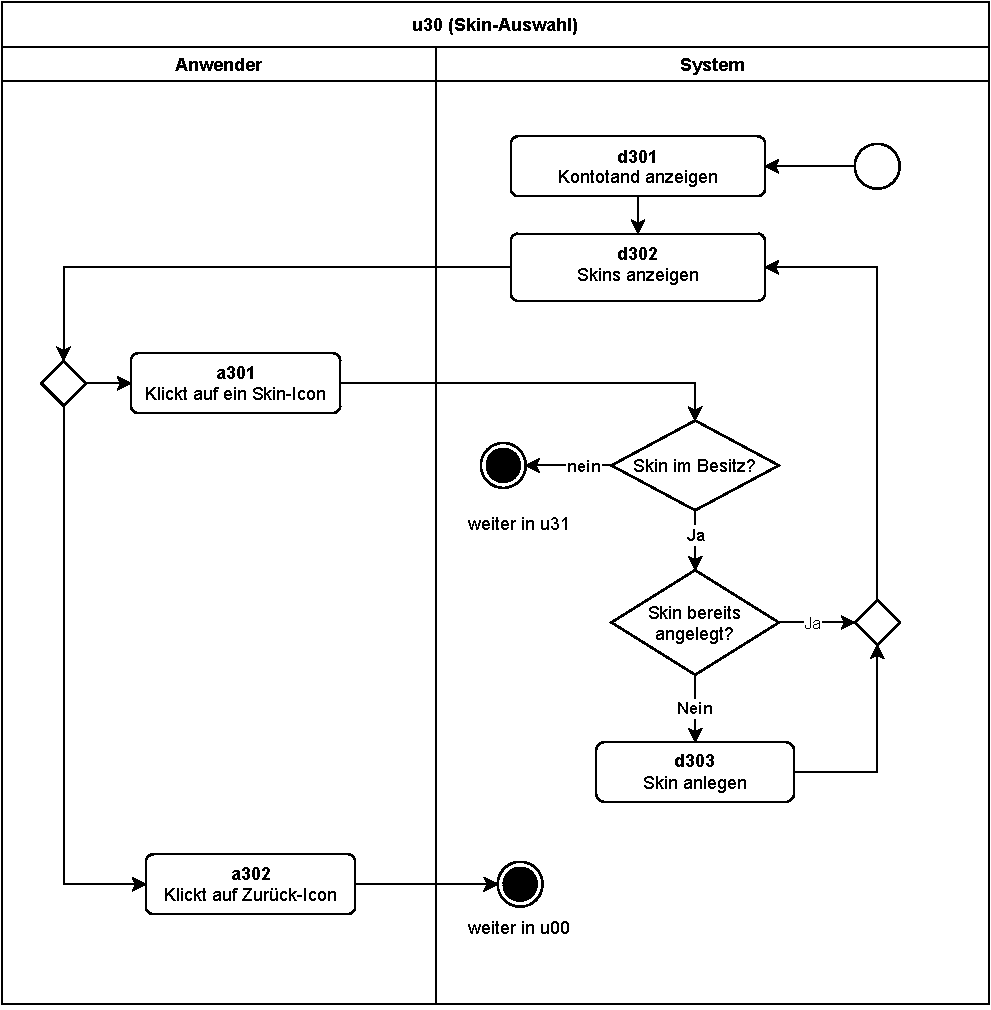
\includegraphics[width=\linewidth]{diagramme/pdf/UML-Activity-u30.pdf}
\captionof{figure}{Aktivität u30 - Skin-Auswahl}\label{fig:dia:skins}
\vspace*{0.5cm}

Klickt der Spieler auf den Skins-Button, so gelangt er auf einen Screen, der ihm alle im Spiel verfügbaren \gls{skin}s des \gls{ball}s, des \gls{tail}s und des Hintergrunds anzeigt. Zusätzlich sieht er hier auch nochmal seinen aktuellen Kontostand. Durch Klicken eines Skin-Icons wird ein Overlay geöffnet, das dem \gls{spieler} die Möglichkeit bietet, den \gls{skin} zu kaufen oder anzulegen. Ist der ausgewählte \gls{skin} bereits angelegt, so wird das Overlay geschlossen und der Spieler kehrt zu der Anzeige aller \gls{skin}s zurück.
\clearpage

\subsubsection{Aktivität u31 - Skin kauf}

\vspace*{1cm}

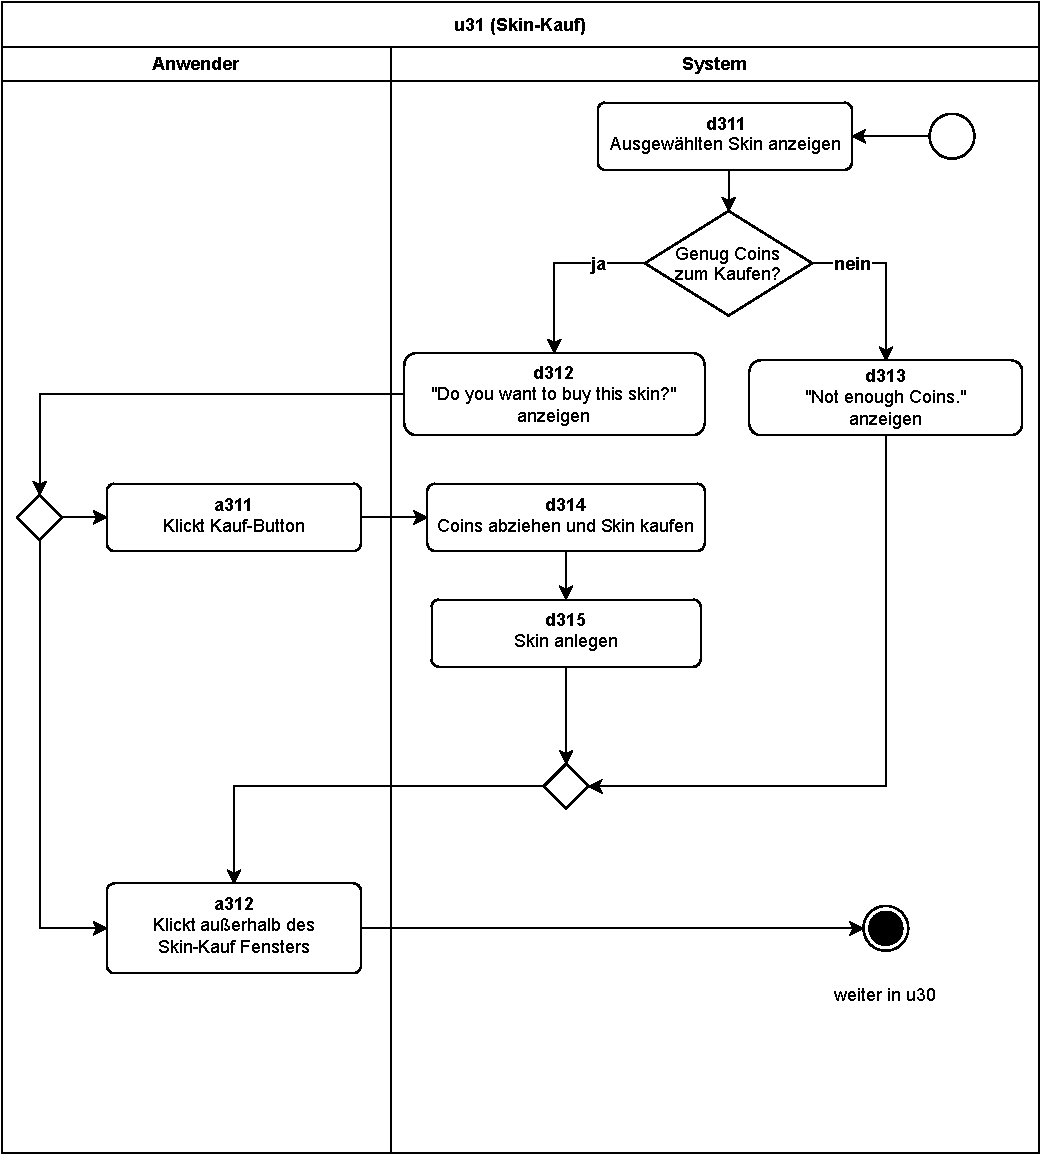
\includegraphics[width=\linewidth]{diagramme/pdf/UML-Activity-u31.pdf}
\captionof{figure}{Aktivität u31 - Skin kauf}\label{fig:dia:skinPurchase}
\vspace*{0.5cm}

Hat der \gls{spieler} einen \gls{skin} ausgewählt, so wird ein Overlay geöffnet. Ist der \gls{skin} noch nicht in seinem Besitz, so wird vom System geprüft, ob genügend Coins für den Kauf des \gls{skin}s vorhanden sind. Ist dies der Fall, so wird die Nachricht „Do you want to buy this skin?“ angezeigt. Entscheidet sich dann der \gls{spieler} disen zu kaufen, so werden die benötigten Coins von seinem Konto abgezogen, der \gls{skin} freigeschaltet und direkt angelegt. 
Fehlen dem \gls{spieler} noch Coins für den \gls{skin}, so zeigt das System die Nachricht „Not enough Coins“ an. Mit einem Klick außerhalb des Overlays kommt der \gls{spieler} dann wieder zurück auf die Anzeige aller \gls{skin}s.

\clearpage

\subsubsection{Aktivität u40 -Credits}

\vspace*{1cm}

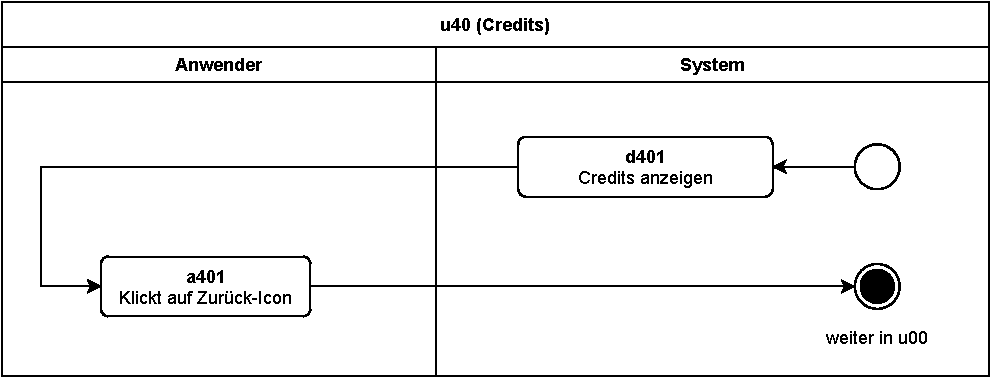
\includegraphics[width=\linewidth]{diagramme/pdf/UML-Activity-u40.pdf}
\captionof{figure}{Aktivität u40 -Credits}\label{fig:dia:credits}
\vspace*{0.5cm}

Bei einem Klick auf den Credits-Button muss das System dem \gls{spieler} die Credits anzeigen. 
Dieser enthält paar Worte der Entwickler und listet alle Mitwirkenden am Spiel auf. 
Der \gls{spieler} hat die Möglichkeit den Credits Screen durch einen Klick auf das Zurück-Icon zu verlassen und das \hyperref[fig:dia:mainMenu]{Hauptmenü} zu erreichen.

\clearpage





